%!TEX root = ../main.tex
%=========================================================

\section{Performance Evaluation}\label{sec:eval}

In  this  section,  we  provide  a  detailed  investigation  of  the performance of the proposed discovery scheme.
We present the performance evalution in three different subsections. 
In the first one we evaluate the performance of our novel waiting function by measuring the ticket table occupancy
according with our design goals and parameters.
The second one is a thorough performance evaluation under different scenarios, including Sybil attacks, of the whole network discovery solution using a peer-to-peer network simulator.
In the third one we include an evaluation using the most used Ethereum client software, Geth~\cite{go-ethereum}, in a testbed scenario.

\subsection{Ticket table occupancy evaluation}

- Ticket table occupancy  and waiting time evaluation

\subsection{Network simulator evaluation}

\sergi{TODO: modify figures with bigger fonts}
\sergi{TODO: registrant distribution is not very readable. probably should be redesign}
\sergi{TODO: Lookup performance should be compared with something. Discv4? }

%\subsubsection{Evaluation Setup}

For the network performance evaluation we extended the existing 
large-scale peer-to-peer network simulatior PeerSim~\cite{p2p09-peersim}.
We implemented the current Discv5 protocol by modyfing the available PeerSim Kademlia implementation with the differences of the Kademlia version used by the Ethereum network, and developing our solution on top of it.

In Table~\ref{tab:param} we show the parameters used in the simulation. 

\begin{table}[!hbt]
\centering
\scriptsize
\begin{tabular}{|c|c|}%|c|c|}
\hline
Parameter     & Value (\%) \\
\hline
\hline
%Network size & 2000 nodes \\%&  0.4321 & 0.8883\\
%\hline
Simulation time & 4 hours \\%& 0.7569 & 0.9959\\
\hline
Kademlia bucket size & 16 \\%& 0.6104 & 0.8515\\
\hline
Kademlia buckets & 17 \\%& 0.8225 & 0.9897\\
\hline
Ticket table bucket size & 5 \\%& 0.8225 & 0.9897\\
\hline
Ticket table buckets & 10 \\%& 0.8225 & 0.9897\\
\hline
Lookup table bucket size & 16 \\%& 0.8225 & 0.9897\\
\hline
Lookup table buckets & 17 \\%& 0.8225 & 0.9897\\
\hline
Registration lifetime & 15 minutes \\%& 0.8225 & 0.9897\\
\hline
Number of topics & 5 \\%& 0.8225 & 0.9897\\
\hline
Number of topics & 5 \\%& 0.8225 & 0.9897\\
hline
Ticket table size & X \\
\hline
Turbulence & X \\%& 0.8225 & 0.9897\\
\hline
\bottomrule
\end{tabular}
\vspace{2mm}
\caption{Evaluation scenario parameters}
\label{tab:param}
\vspace{-0.05in}
\end{table}



%\begin{table}[!hbt]
%\centering
%\scriptsize
%\begin{tabular}{|c|c|}%|c|c|}
%\hline
%Topic & 500 Nodes & 1000 Nodes & 5000 nodes & 10000 nodes \\
%\hline
%\hline
%T1 & 500 nodes & 1000 nodes & 5000 nodes & 10000 nodes \\%&  0.4321 & 0.8883\\
%\hline
%T2 & 1272 nodes \\%& 0.7569 & 0.9959\\
%\hline
%T3 & 803 nodes \\%& 0.6104 & 0.8515\\
%\hline
%T4 & 496 nodes \\%& 0.8225 & 0.9897\\
%\hline
%T5 & 218 nodes \\%& 0.8225 & 0.9897\\
%\hline
%\bottomrule
%\end{tabular}
%\vspace{2mm}
%\caption{Nodes per topic}
%\label{tab:nodes}
%\vspace{-0.05in}
%\end{table}


%\subsubsection{Results}

%\paragraph{\bf{Active registrations}:}

\subsubsection{Performance Results}


%\paragraph{Ticket registrations:

In Figure~\ref{fig:regs} we observe the average active registrations in the system per topic. 
We can observe nodes for all topics are able to place a substantial amount of registrations, even the less popular topics. 
As number of nodes increase in the network, we can observe the differences between registrations per topic are reduced. 
Actually, it can be observed the most popular topic (t1) is able to place less registrations than t2. 
This is caused by the fact that with more nodes trying to register for the same topic, waiting times increase and therefore is more difficult to register.

In Figure~\ref{fig:util} we observe the average utilisation of the ticket table for all nodes.
We can observe since t1 places less registrations the occupancy for t1 in the tables is less than t2. We can also observe the
overall utilisation does not reach 50\%. 
This is caused by the fact that the waiting time increase does not allow tables to reach the limit. 



\sergi{TODO: change Log scale for fig \ref{fig:regs}}
\begin{figure}[!h]
\centering
\subfigure[{Active registrations}]{
\includegraphics[width=0.225\textwidth]{img/eval/registration_origin.png}
\label{fig:regs}
} 
\hspace{-0.25cm}
\subfigure[{Storage utilization}]{
\includegraphics[width=0.225\textwidth]{img/eval/storage_utilisation.png}
\label{fig:util}
}
 \caption{Ticket registrations} 
\label{fig:registrations}
\vspace{-0.15in}
\end{figure}   

%\begin{figure}[h!]
%\centering
%%\epsfig{file=imgs/eval/scen5.pdf, width=0.45\textwidth}
%\includegraphics[width=0.225\textwidth]{img/eval/registration_origin.png}
%\caption{Registrations}
%\label{fig:regs}
%\vspace{-0.15in}
%\end{figure}

%\paragraph{\bf{Network load}:}
\sergi{TODO: change Log scale for fig \ref{fig:messages}}
In Figure~\ref{fig:messages}~and~\ref{fig:msg_distr} we can observe the traffic load generated in the network.
In Figure~\ref{fig:messages} we observe most of the messages are ticket requests/replies, and the subsequent registration request/replies
after receiving a ticket from a node. 
This is caused by the fact that nodes are constantly registering dynamically. 
In Figure~\ref{fig:msg_distr} the messages received distribution. 
We can observe some nodes receive much more messages.
This is caused by the bucket ndoe distributiong, where nodes with identifiers close to topic hash ids receive more initial tickets requests because there are less.
However, we can see the number of messages received does not exceed X times the average value of the messages received. 
Moreover, we can also observe with the increase of nodes in the network, the load that these nodes receive does not increase in the same way. 
Therefore, the system is able to scale without danger of overloading some of the nodes of the network.

\begin{figure}[!h]
\centering
\subfigure[{Number of messages}]{
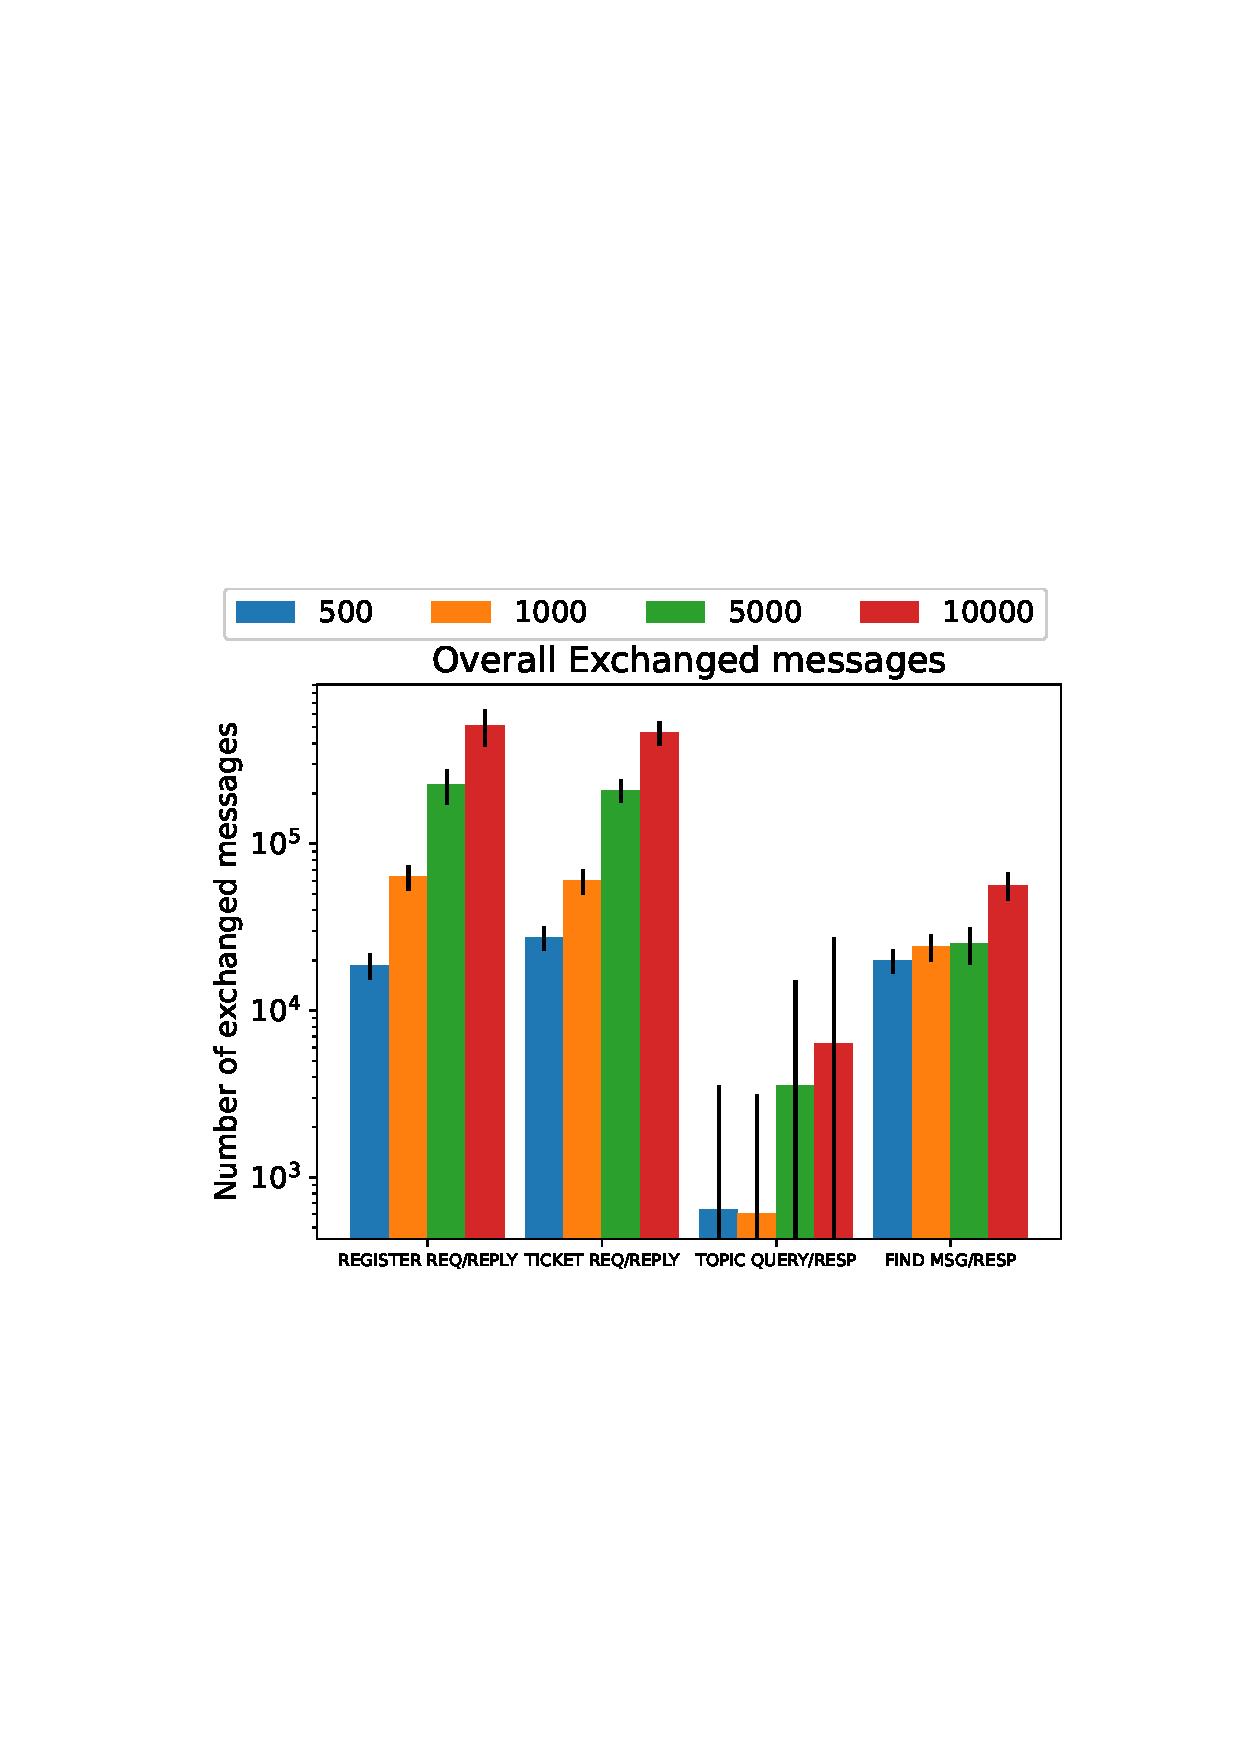
\includegraphics[width=0.225\textwidth]{img/eval/message_quantity.png} 
\label{fig:messages}
} 
\hspace{-0.25cm}
\subfigure[{Message distribution}]{
\includegraphics[width=0.225\textwidth]{img/eval/messages_received2.png} %\hspace{-1.5em}%
\label{fig:msg_distr}
}
 \caption{Traffic load} 
\label{fig:traffic}
\vspace{-0.15in}
\end{figure}   

%\paragraph{\bf{Discovery performance}:}

\begin{figure}[!h]
\centering
\subfigure[{Registrant discovery distribution}]{
\includegraphics[width=0.225\textwidth]{img/eval/registrant_distribution.png} 
\label{fig:reg_disc}
} 
\hspace{-0.25cm}
\subfigure[{Time between registration and first discovery}]{
\includegraphics[width=0.225\textwidth]{img/eval/min_time_discovery.png} %\hspace{-1.5em}%
\label{fig:timedisc}
}
 \caption{Discovery} 
\label{fig:discovery}
\vspace{-0.15in}
\end{figure}   

\paragraph{\bf{Lookup performance}:}

\begin{figure}[h!]
\centering
%\epsfig{file=imgs/eval/scen5.pdf, width=0.45\textwidth}
\includegraphics[width=0.35\textwidth]{img/eval/lookup_hopcount.png}
\caption{Lookup hopcount}
\label{fig:hopcount}
\vspace{-0.15in}
\end{figure}

\subsubsection{Sybil Attacks}


\begin{figure}[!h]
\centering
\subfigure[{Time to register}]{
\includegraphics[width=0.225\textwidth]{img/eval/registrant_distribution.png} 
\label{fig:reg_disc}
} 
\hspace{-0.25cm}
\subfigure[{Lookup hopcount}]{
\includegraphics[width=0.225\textwidth]{img/eval/min_time_discovery.png} %\hspace{-1.5em}%
\label{fig:timedisc}
}
 \caption{Discovery} 
\label{fig:discovery}
\vspace{-0.15in}
\end{figure}   


\paragraph{\bf{Topic Eclipse Attack:}}

%- malicious registrations
%
%- eclipsed nodes
%
%- time to register / time to discovery
%
%- hopcount 

\paragraph{\bf{Denial of Service Attack: random topic attack and dos attack}}



\begin{figure}[!h]
\centering
\subfigure[{Time to register for Non-response DoS Attack}]{
\includegraphics[width=0.225\textwidth]{img/eval/avg_time_register_dos.png} 
\label{fig:reg_disc}
} 
\hspace{-0.16cm}
\subfigure[{Lookup hopcount for Non-response  DoS Attack}]{
\includegraphics[width=0.225\textwidth]{img/eval/min_time_discovery_dos.png} %\hspace{-1.5em}%
\label{fig:timedisc}
}
 \caption{Registration and Discovery performance for the Non-response DoS Attack} 
\label{fig:discovery}
\vspace{-0.15in}
\end{figure}   


\begin{figure}[!h]
\centering
\subfigure[{Time to register for the random topic  DoS Attack}]{
\includegraphics[width=0.225\textwidth]{img/eval/avg_time_register_randomtopic.png} 
\label{fig:reg_disc}
} 
\hspace{-0.16cm}
\subfigure[{Lookup hopcount for the random topic  DoS Attack}]{
\includegraphics[width=0.225\textwidth]{img/eval/lookup_hopcount_randomtopic.png} %\hspace{-1.5em}%
\label{fig:timedisc}
}
 \caption{Registration and Discovery performance for the random topic  DoS Attack} 
\label{fig:discovery}
\vspace{-0.15in}
\end{figure}   


%- active registrations
%
%- time to register / time to discovery
%
%- hopcount 

\subsection{Testbed evaluation}

"Geth"~\cite{go-ethereum} performance evaluation: \hl{TBC}.
